\documentclass[conference]{IEEEtran}
%\documentclass[sigconf]{acmart}
\makeatletter
\def\ps@headings{%
\def\@oddhead{\mbox{}\scriptsize\rightmark \hfil \thepage}%
\def\@evenhead{\scriptsize\thepage \hfil \leftmark\mbox{}}%
\def\@oddfoot{}%
\def\@evenfoot{}}
\makeatother
\pagestyle{empty}
\usepackage{url}
\usepackage{graphicx,subfigure}
\usepackage{epstopdf}
\usepackage{amsmath}
\usepackage{algorithm}
\usepackage{algpseudocode}
\usepackage{amsmath}
\usepackage{amssymb}
\usepackage{amsthm}
\usepackage{epsfig}
\newtheorem{theorem}{Theorem}
\renewcommand{\algorithmicrequire}{\textbf{Input:}} % Use Input in the format of Algorithm
\renewcommand{\algorithmicensure}{\textbf{Output:}} % Use Output in the format of Algorithm
\usepackage{amsfonts}
%\newtheorem{theorem}{Theorem}[section]
\newtheorem{mydef}{Definition}[section]
%\newtheorem{lemma}{Lemma}[section]
\usepackage{multirow}
\usepackage{color}
\usepackage{array}
\usepackage{listings}
\usepackage{hyperref}
\usepackage[underline=true]{pgf-umlsd}
\newcommand{\tabincell}[2]
{\begin{tabular}
		{@{}#1@{}}#2\end{tabular}}
\usepackage{setspace}
\renewcommand{\labelitemi}{$\vcenter{\hbox{\tiny$\bullet$}}$}


\hyphenation{op-tical net-works semi-conduc-tor}




\begin{document}
\graphicspath{{photos/},{../diagrams/}}



\title{Team 2 \linebreak
 Chicago Car Accidents Assessment Utilizing Clustering Analysis}

\author{\IEEEauthorblockN{1\textsuperscript{st} Hodgetts, Michael }
\IEEEauthorblockA{\textit{Electrical Engineering Dept} \\
\textit{EE-695 - Machine Learning }\\
Hoboken, NJ \\
mhodgetts@comcast.net}
\and
\IEEEauthorblockN{2\textsuperscript{nd} Paladugu, Rithvika}
\IEEEauthorblockA{\textit{Computer Engineering} \\
\textit{EE 695 - Machine Learning}\\
Hoboken, NJ \\
paldugurithvika@gmail.com}
\and
\IEEEauthorblockN{3\textsuperscript{rd} Nathan, Barry}
\IEEEauthorblockA{\textit{dept. name of organization (of Aff.)} \\
\textit{EE-695 - Machine Learning}\\
Hoboken, NJ \\
nate.b4rry@gmail.com}
}

\maketitle


\begin{abstract}
Practice as a team to analyse unsupervised data by exploring various clustering methods (k-means, k-modes, kprototype, Gaussian and DBSCAN) on Chicago Accident database.
\end{abstract}

\section{Introduction}
Utilizing two datasets from Chicago Department website (Crashes and People related to Crashes), we like to find areas/neighborhoods 
within the city that have different characteristics in terms of the attributes available.  Dataset is large (750K rows) so we decided to look at only 2 years 
(2021 and 2022) which reduces to about 250K.  There is a good amount of prep to get data suitable for cluster analysis (ETL, Hot Encoding, data cleanup)
We will try at least 3 different methods and compare the results. Since the data his mixed we have limited methods to do cluster analysis.  We'll choose the better model and create an optimum number of clusters to analyze.  We will illustrate some of the main 
differences these assigned clusters present. Provide a summary of each cluster characteristics to illustrate the main differences between them.  You'll see in this report we have already started this plan.

\section{Related Work}
There are many examples on how clustering solves problems in various business use cases.  Segmentation analysis, anomoly detection and a form of classification are some of the use cases. The analysis here could be useful to identify hot areas of accidents due to poor signage, road conditions, and other conditions that could be 
improved to reduce accidents or injuries in the Chicago area.  Practicing how to get meaningful insights is essential in the business world. 


\section{Our Solution}
Since the data is large and has many attributes (both numerical and categorical), reducing the number of attributes will be critical.  Also, minimizing the number of clusters needed is beneficial to ensure each cluster has meaningful differences and similar volume. Heatmaps showing differences will be 
provided to help show major allocation of attributes to each cluster. Another issue is we have a lot of category data as well as continous.  k-modes was explored first since it handles categorical data and kmeans covers numerical.  K-Prototypes covers both at the same time.  We tried to use Gaussian Mixture but that seems to not be appropriate and gave us unusual results.  Another method is DBSCAN which can handle hot encoding but so far find it difficult to gain the necessary clusters needed, very sensitive to noise (EPS) and size of data.  kprototype so far has the best results with the mixed data.  We will show Heatmaps to illustrate our results and provide summary description of the final clustering results.

\subsection{Description of Dataset}
The dataset can be found here: \href{https://data.cityofchicago.org/Transportation/Traffic-Crashes-Crashes/85ca-t3if}{Chicago Crashe Data}, Two datasets; one for crashes in Chicago and the other are the people characteristics of those crashes.  The 'Crash ID' is the key attribute to join the 2 datasets.  We reduced the size to only years 2021 and 2022 which still leaves about 250K rows and 68 columns.  We used Knime (ETL software) to help do this join and ensure it was properly achieved.  Data had very few problems with missing data but we removed as necessary or added average values as needed. We separated the dataset into two parts, categorical and numerical.  Performed Hot Encoding
on the categorical and scaling on the numberical (0,1), then combined them back together as one file.  New Shape of the file is now  248K by 111 columns with hot encoding. We created another dataset for k-prototypes which has 31 columns based on what attributes we deemed valuable.  Pie charts were useful in this particular dataset since most attributes are categorical.  Many Attributes had too many categories that represented less than 1 percent of the size so we create algorithm to gather them up into a 'Remainder' for each category to help reduce the number of hot columns needed. \linebreak
Below is the list of columns we are working with in the dataset.  Some have been removed since they will not contribute to the model performance.
\begin{figure}[!h]
	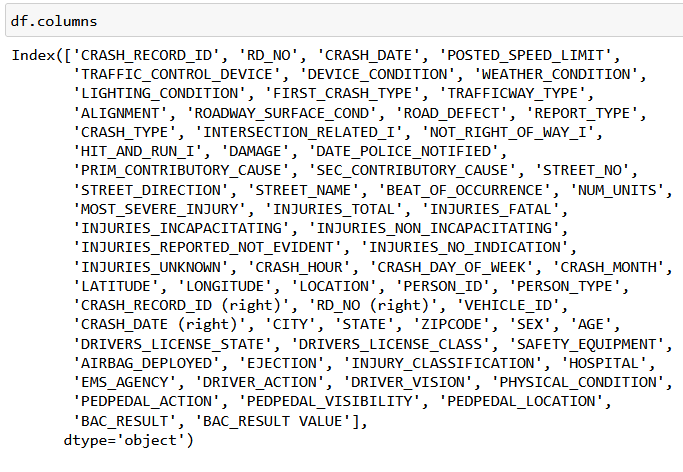
\includegraphics[width=\linewidth]{Chicago_Column.png}
	\caption{Chicago Dataset}
	\label{fig: Chicago Dataset for Crashes and People involved}
 \end{figure}

\textbf{EDA} \linebreak
Here we show a sampling of some of the attributes classes for the categorical data and numerical.  There are many columns so we will just show a sample of some. You can see more in the code readout. 
\begin{figure}[!h]
	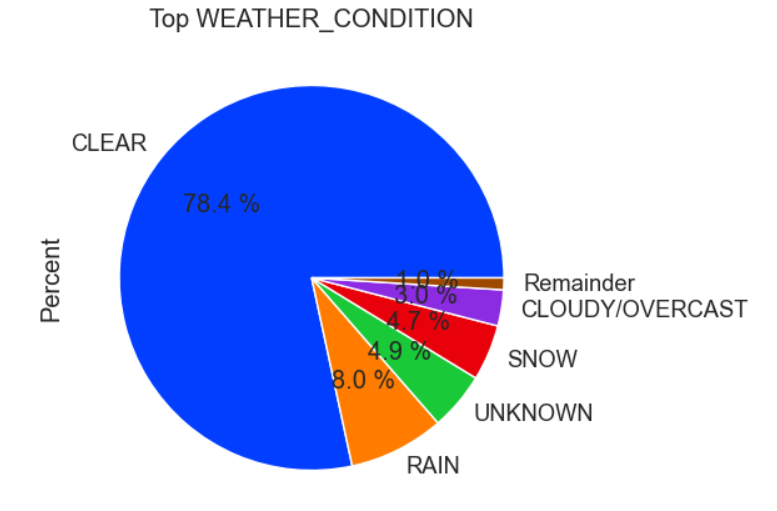
\includegraphics[width=\linewidth]{TOP_WEATHER_CONDITION_PIE.png}
	\caption{Categorical Pie Charts (Sampling View)}
	\label{fig: Top_Weather_Condition Pie chart}
 \end{figure}

 

 \begin{figure}[!h]
	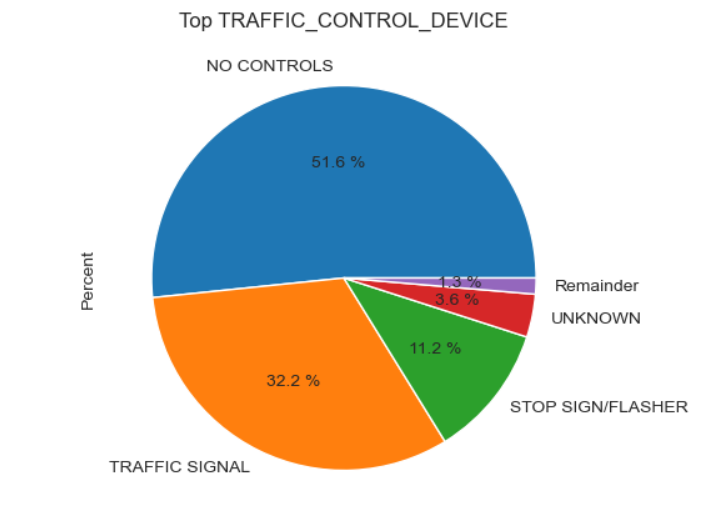
\includegraphics[width=\linewidth]{Traffic_Control_Pie.png}
	\caption{Traffic_Control_Pie}
	\label{fig: Traffic_Control_Pie}
 \end{figure}
 Here are some of the numeric attributes to examine
 \begin{figure}[!h]
	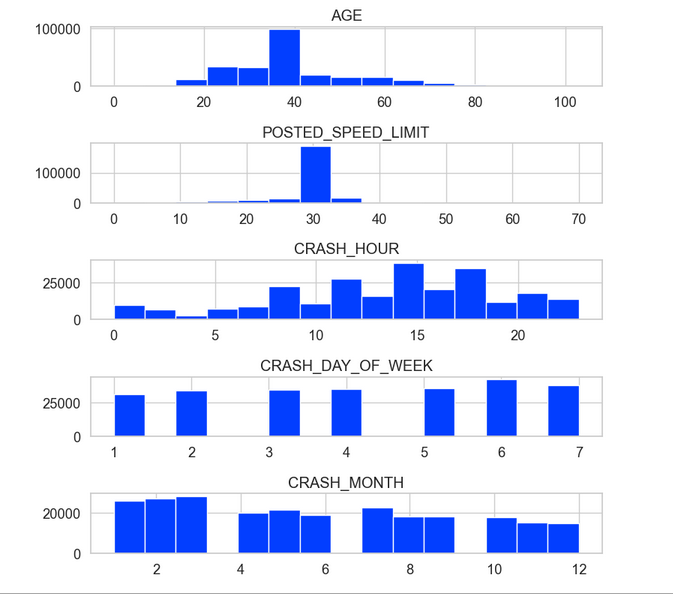
\includegraphics[width=\linewidth]{Numerical_Hist.png}
	\caption{Numeric Histograms (Sampling View)}
	\label{fig: Numeric Histograms}
 \end{figure}

 note:

\subsection{Machine Learning Algorithms}
Our data is raw and has no classification or specific purpose so it lends itself to utilize unsupervised data techniques. 
We explored K-modes, kmeans, kprototype and DBSCAN and will investigate other possible methods to find insights. kprototype is our best hope so far to get good results since 
it handles both categorical and numeric attributes.  Kmodes can only handle category and kmeans does numerical. Noticed Kprototype takes a very long time to process the model.  Elbow curve took over 24 hours. Since we have a large dataset, training take a good length of time for all model types.  We created elbow curves for both K-modes and Kprototypes in the figures below:  
\begin{figure}[!h]
	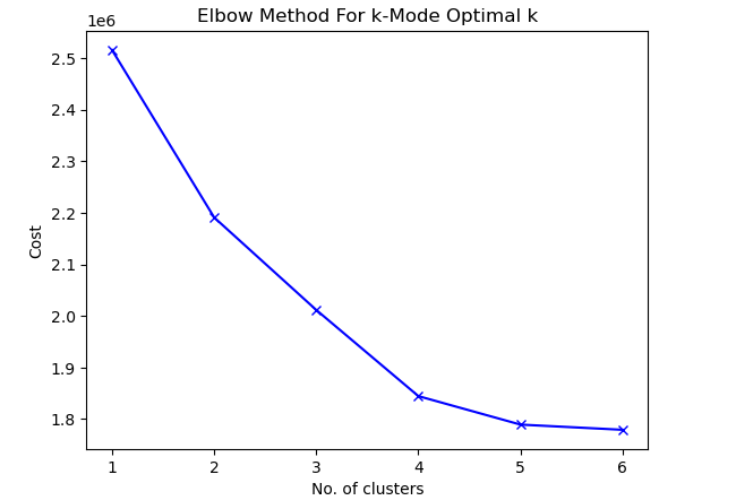
\includegraphics[width=\linewidth]{k_mode_elbow.png}
	\caption{k-means}
	\label{fig: kmean elbow chart}
 \end{figure}
 \ linebreak
 \begin{figure}[!h]
	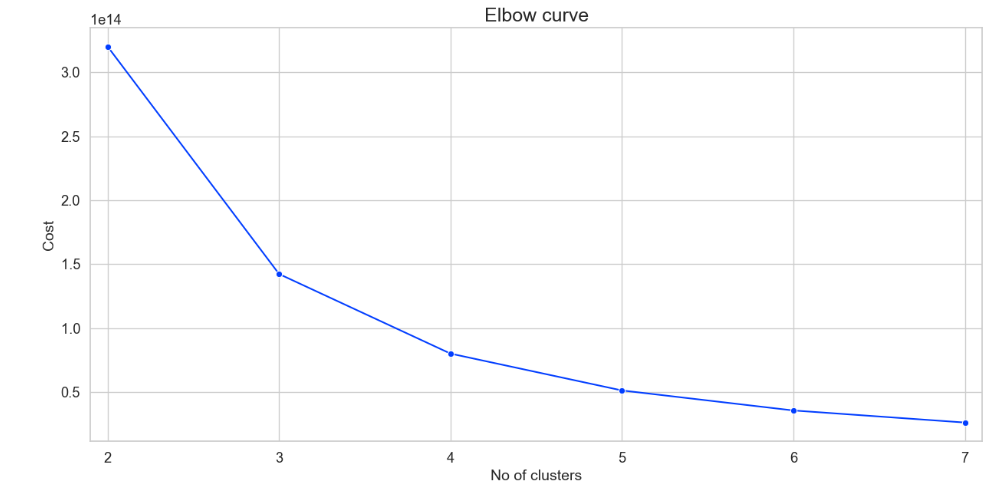
\includegraphics[width=\linewidth]{KPrototype_Elbow.png}
	\caption{k-prototype}
	\label{fig: kprototype elbow chart}
 \end{figure}

From figures 2 and 3 you can see 4 clusters would be reasonable.  We currently picked 4 clusters as a start. The difficulty is assessing the 
cluster characteristics with so many attributes.  We did some Chi Testing on the attributes to find any that were not relevate but all picked were significant.
\begin{figure}[!h]
	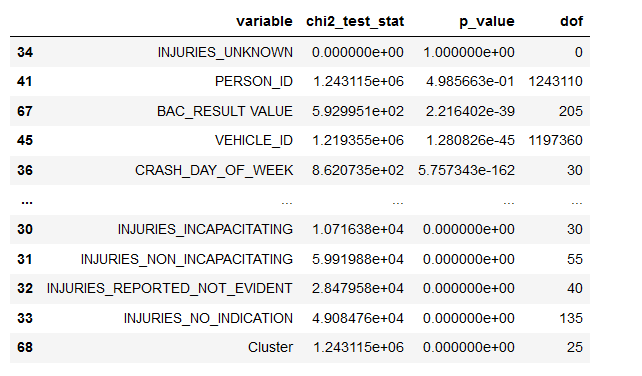
\includegraphics[width=\linewidth]{Chi Square.png}
	\caption{Chi Square Testing View}
	\label{table: Chi Square Testing View}
\end{figure}
We uUtilized pspark to use groupby by clusters by percent of occurence to see what patterns emerge.  We may have to build this view outside of Python to get a good illustrative view ith excel.  At the current time, we're assessing how to decribe these these clusters and find recommendations to provide back to the city of Chicago. This figure below issustrates the comparison we are doing with 4 clusters verses the categorical columns.  You can see clearly differences in of how the clustering divided up the percent allocation. Percent allocation is based total population so we can compare to each different attribute.  Will do the same for the numerical but it will look a little different since we will use averages.
\begin{figure}[!h]
	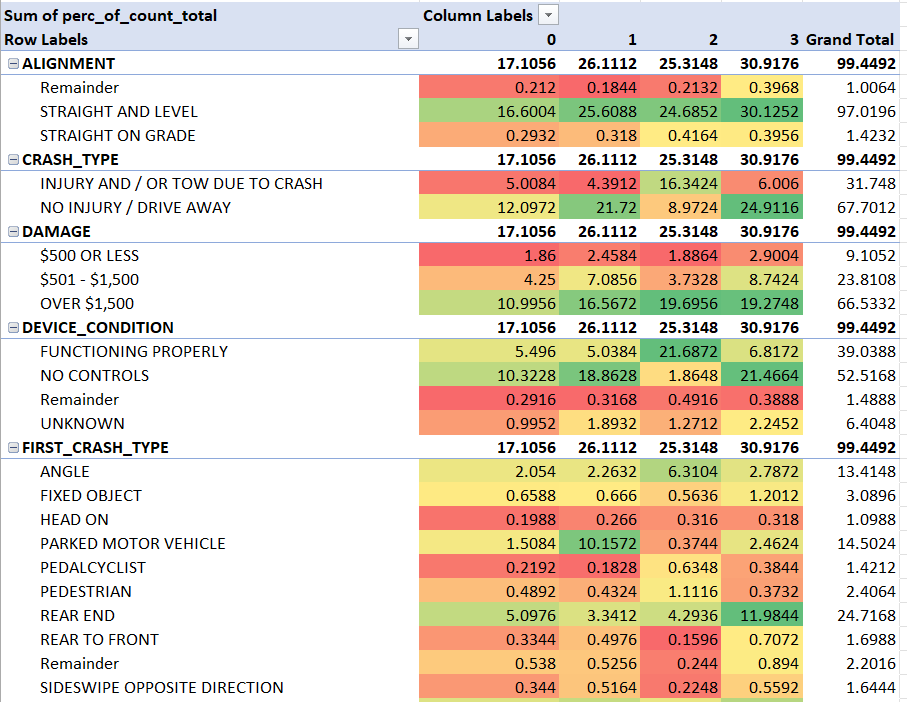
\includegraphics[width=\linewidth]{KP_Percent_ALL.png}
	\caption{Example of Cluster Heatmap for Categorical Attributes }
	\label{fig: Example of Cluster Heatmap for Categorical Attributes (4 Clusters)}
\end{figure}
2

\section{Comparison}  
Gaussian clustered results didn't look correct since the majority of the volume was placed into one cluster, we think this is because it can't handle or interpret hot encoding or dummy variable too well.  Kmodes and Kprototype gave similar results. 
report.  Also DBSCAN was very senstive to EPS and Samples and could not achieve 4 clusters but only 3 with a majority of volume in one cluster alone.  We will continue to examine if we can resolve this.
We will add to this section in our final.

\section{Future Directions}
We still need to try other methods and see if the allocations are significantly different.  We'll describe each cluster characteristics in more detail.
We like to show so mapping features of how the clusters map over Chicago but find this difficult so far to accomplish.  There another method call Squeezer which can be used with mixed data but has little documentaion.  Deep learning techniques utilaing autoencoders can be examined.  We'll add to this section for our final report

\section{Conclusions}
We'll add our conclusions at the final report
 

\bibliographystyle{IEEEtran}
\bibliography{}
1) https://scottmduda.medium.com/categorical-clustering-of-pittsburgh-car-accidents-using-k-modes-7c842cc15d87 \linebreak
2) https://data.cityofchicago.org/Transportation/Traffic-Crashes-Crashes/85ca-t3if \linebreak
3) https://www.freecodecamp.org/news/8-clustering-algorithms-in-machine-learning-that-all-data-scientists-should-know/  \linebreak
4) https://scikit-learn.org/stable/auto_examples/cluster/plot_dbscan.html \linebreak
5) https://antonsruberts.github.io/kproto-audience/ \linebreak

\end{document}


